\chapter{Experiments and Results}


\section{Experiments}

\iffalse
SVM-Regression
Random-Forest Regression
Deep Learning Network

Neural Net Sequence Embeddings
One-Hot Encodings
Modfied n-grams skip-grams
\fi

The focus of the experiments are concentrated on the properties of protein as they have complex structures. The binding of protein and drug depend on various attributes of protein like acidity, hydrophobicity, binding pockets etc and the structure of drug. The attributes are quite closely related to primary and secondary structure of protein themselves. Therefore, our model aims to relate all these multiple components with matrix representation and confirming to Figure ~\ref{fig:kiba_drug_protein} prediction.

\subsection{Features Selection}
\subsubsection{Primary Feature Selection}
The sequence information of drugs and proteins live in their canonical form. 
% Exploring to the other embedding technique used in language theory, the modified N-Grams Skip-Grams (m-NGSG) was supposed to undertake the mutational agreements when the proteins and drug interaction was brought in question. However, it fared quite badly than the Neural Net Sequence Embeddings. Mostly the issue can be related to that if the algorithm misses the tight relationship among the amino-acid neighborhood, then the protein with different structure may seem to act similarly: a strong disagreement on principle that certain proteins with slight modification on the sequence have different functional and chemical properties. It could still be used for Poisson-Hidden Markov Model for some other properties, but primary encodings can't be relied on m-NGSG. 
Therefore we relied on Neural Net Sequence Embedding technique to form the primary representation. Both protein and drug were converted to Embedding vectors after creation of their labelled encodings. 

\subsubsection{Secondary Features Selection}
These are the structural components of protein especially related to alpha and beta strands of Protein segments. All the protein Sequences are subjected to Equation~(\ref{eq:pssm}) from the labelled encodings. The \acrshort{pssm} matrix is calculated using PSI-BLAST\cite{Schaffer2001}. Then all the testing protein sets are evaluated with the resultant PSSM to form a new PSSM matrix specific to the testing protein. Thus, we expect to explore how proteins relate with the interaction experiments with the protein domain. From the \acrshort{pssm}, we evaluate the other evolutionary and distance vectors using equations \ref{eq:rpt}, \ref{eq:pssmddt}, \ref{eq:pssmsdt} and \ref{eq:edt}.

\subsection{Implementation}
% We explore basically the following algorithms for analyses on protein-drug interactions:


\subsubsection{Stacked Features}
Basically, we implement the architecture in Figure ~\ref{fig:dlm} for our model design. It is implemented in Python using the TensorFlow framework consisting of keras. The training contained of 200 epochs. The learning rates and early stopping were manipulated in the training process by using keras callback functions. The training and testing was done using a 5-fold cross-validation set prepared manually. To evaluate the performance of the model, we used concordance index(CI)\cite{Xu2015} as defined by equation~\ref{eq:ci}:
\begin{equation}
    CI = \frac{1}{Z} \sum_{\delta_i > \delta_j} h(b_i - b_j)
    \label{eq:ci}
\end{equation}
where $b_i$ is the prediction value for higher affinity $\delta_i$ and $b_j$ is the prediction value for smallery affinity $\delta_j$, $Z$ is the normalization constant and $h(m)$ is the unit step function:
\begin{equation} h(x) = 
    \begin{cases}
        1,& \quad {if x>0} \\
        0.5, & \quad{ if x=0 } \\
        0, & \quad{if x<0} \\
    \end{cases}
\end{equation}

\section{Results}

The deep learning method was implemented with various filter sizes of Convolutional Layer of Protein and Drugs. Only the comparable results have been shown in Table \ref{table:results}. The training and validation plots under different settings is clearly shown by Figure \ref{fig:ci_curve}. The different settings are:
\begin{itemize}
    \item Setting 1 (S1): The validation proteins and drugs appear in training set.
    \item Setting 2 (S2): The validation Protein is seen in training set but validation drugs aren't present while training.
    \item Setting 3 (S3): The validation Protein is absent in training set but validation drugs are present in training set.
    \item Setting 4 (S4): The validation Protein and Drugs don't appear in training set
\end{itemize}

\begin{table}[H]
    \centering
    \caption{Experiments results under different settings (S1, S2, S3, S4)}
    \begin{tabular}{|l|c|c|c|c|c|c|}
    \hline 
    
     S.No. & Drug Smiles & FASTA & Setting & CI-val & MSE & CI-train \\ 
     & Window Size &  Window Size  &  & &  &  \\  \hline 
    1 & 4 & 8 & 1 & 0.813936 & 0.811580 & 0.893064 \\ \hline
    2 & 4 & 12 & 1 & 0.810844 & 0.809919 & 1.285271 \\ \hline
    3 & 8 & 8 & 1 & 0.873094 & 0.873648 & 0.177053 \\ \hline
    4 & 8 & 12 & 1 & 0.807230 & 0.806509 & 1.056755 \\ \hline
    \\ \hline
    1 & 4 & 8 & 2 & 0.788051 & 0.789266 & 0.678707 \\ \hline
    2 & 4 & 12 & 2 & 0.802355 & 0.802892 & 0.360900 \\ \hline
    3 & 8 & 8 & 2 & 0.803720 & 0.806808 & 0.792821 \\ \hline
    4 & 8 & 12 & 2 & 0.803853 & 0.805306 & 0.672790 \\ \hline
    \\ \hline
    1 & 4 & 8 & 3 & 0.815181 & 0.815076 & 1.562749 \\ \hline
    2 & 4 & 12 & 3 & 0.805739 & 0.806455 & 1.541746 \\ \hline
    3 & 8 & 8 & 3 & 0.813063 & 0.813148 & 1.259206 \\ \hline
    4 & 8 & 12 & 3 & 0.824767 & 0.825603 & 1.396765 \\ \hline
    \\ \hline
    1 & 4 & 8 & 4 & 0.803982 & 0.804584 & 0.412271 \\ \hline
    2 & 4 & 12 & 4 & 0.805961 & 0.807584 & 1.510426 \\ \hline
    3 & 8 & 8 & 4 & 0.815464 & 0.816097 & 1.614631 \\ \hline
    4 & 8 & 12 & 4 & 0.787073 & 0.787795 & 0.485298 \\ \hline
    
    
    \end{tabular}
    \label{table:results}
\end{table}

\section{Analysis}
The Table \ref{table:results} shows that the optimal filter window size under all settings can be chosen equal to 8 for both drugs and proteins. The highest C-Index Score of (87.30\%) was obtained under Setting 1 when both the drugs and proteins were present in the validation set and training set. This can also be better realized visually from Figure \ref{fig:ci_curve}.
 
\begin{figure}[H]\centering
    \subfloat[][Setting 1]{
        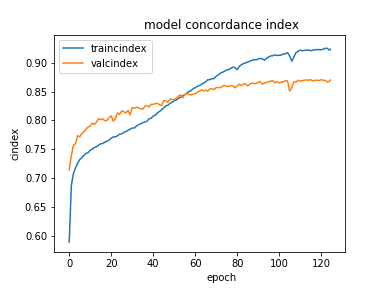
\includegraphics[width=.45\textwidth]{mainmatter/4-Results/images/S1_CI.png}
    }
    \qquad
    \subfloat[][Setting 2]{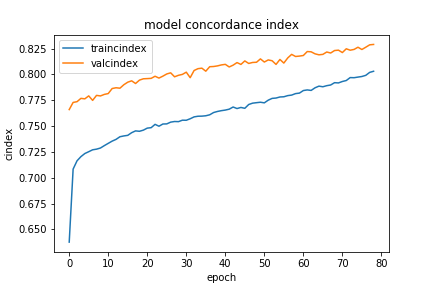
\includegraphics[width=.45\textwidth]{mainmatter/4-Results/images/S2_CI.png}}
    \qquad
    \subfloat[][Setting 3]{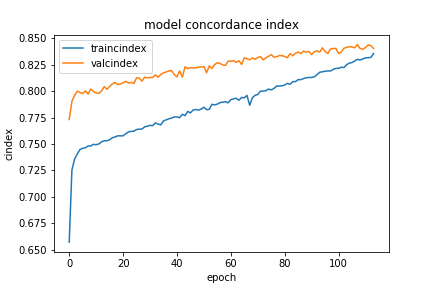
\includegraphics[width=.45\textwidth]{mainmatter/4-Results/images/S3_CI.png}}
    \qquad
    \subfloat[][Setting 4]{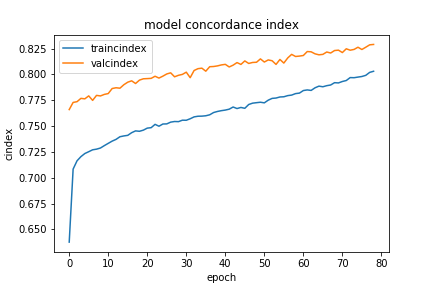
\includegraphics[width=.45\textwidth]{mainmatter/4-Results/images/S4_CI.png}}
    \caption{Plot of Training-Validation C-Index Scores over various Settings}
    \label{fig:ci_curve}
\end{figure}

\section{Conclusion}
The training of the model proved a better choice as we added the new feature dimension for proteins to get a generalization of all the feature sets extracted from the drug and protein sequence.

\begin{figure}[H]
    \subfloat[Training Actual Scores]{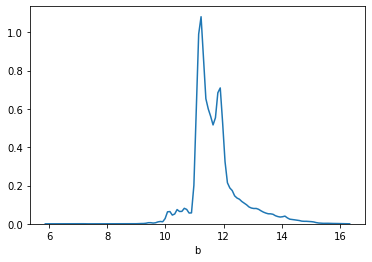
\includegraphics[width=.3\textwidth]{mainmatter/4-Results/images/train_y.png}}
    \subfloat[Training Predicted Scores]{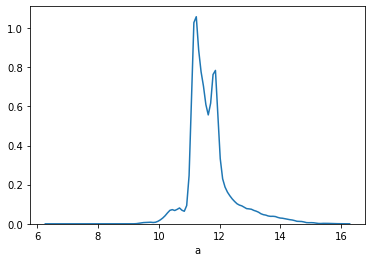
\includegraphics[width=.3\textwidth]{mainmatter/4-Results/images/pred_train_y.png}}
    \subfloat[Training Scores Difference]{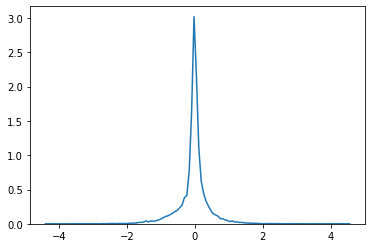
\includegraphics[width=.3\textwidth]{mainmatter/4-Results/images/train_diff.png}}
    \caption{Training Results based on KIBA Score Prediction}
    \label{fig:pred_train}
\end{figure}

\begin{figure}
    \centering
    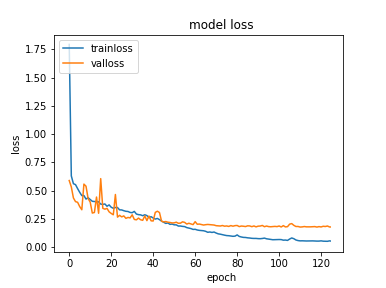
\includegraphics[width=.8\textwidth]{mainmatter/4-Results/images/S1_loss.png}
    \caption{Training and Validation Loss Plot of Setting 1 (S1) with Filter Size = 8}
    \label{fig:train_val_loss_plot}
\end{figure}

Similarly, the prediction scores and actual scores for validation sets is shown in Figure ~\ref{fig:val_train}
\begin{figure}[H]
    \subfloat[Testing Actual Scores]{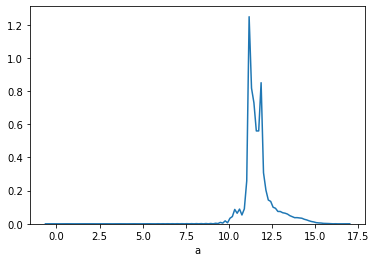
\includegraphics[width=.3\textwidth]{mainmatter/4-Results/images/val_y.png}}
    \subfloat[Testing Predicted Scores]{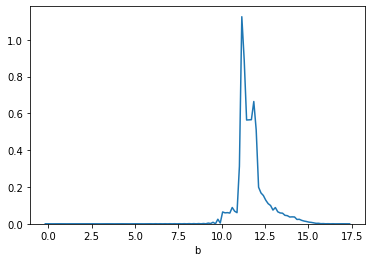
\includegraphics[width=.3\textwidth]{mainmatter/4-Results/images/pred_val_y.png}}
    \subfloat[Testing Scores Difference]{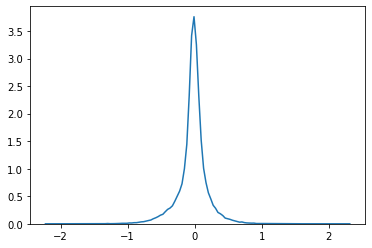
\includegraphics[width=.3\textwidth]{mainmatter/4-Results/images/val_difference.png}}
    \caption{Testing Results on KIBA score Prediction}
    \label{fig:val_train}
\end{figure}

\iffalse The similarity measures are evaluated using \cite{Cock2009}. \fi

\iffalse
The accuracy plots and cindex plots are shown in Figure ~\ref{fig:results}
\begin{figure}
    
\end{figure}

% Setting No. 4 Janahit
P1 = 0,  P2 = 0, P3 = 0, Fold = 2, CI-i = 0.804584, CI-ii = 0.803982, MSE = 0.412271
P1 = 0,  P2 = 0, P3 = 1, Fold = 2, CI-i = 0.807584, CI-ii = 0.805961, MSE = 1.510426
P1 = 0,  P2 = 1, P3 = 0, Fold = 2, CI-i = 0.816097, CI-ii = 0.815464, MSE = 1.614631
P1 = 0,  P2 = 1, P3 = 1, Fold = 2, CI-i = 0.787795, CI-ii = 0.787073, MSE = 0.485298
P1 = 0,  P2 = 0, P3 = 0, Fold = 1, CI-i = 0.829441, CI-ii = 0.829419, MSE = 0.529846
P1 = 0,  P2 = 0, P3 = 1, Fold = 1, CI-i = 0.805457, CI-ii = 0.805507, MSE = 0.810648
P1 = 0,  P2 = 1, P3 = 0, Fold = 1, CI-i = 0.816638, CI-ii = 0.817120, MSE = 0.922689
P1 = 0,  P2 = 1, P3 = 1, Fold = 1, CI-i = 0.829794, CI-ii = 0.829780, MSE = 0.271460
% Setting No. 2 alwaysgetwithanup
P1 = 0,  P2 = 0, P3 = 0, Fold = 0, CI-i = 0.788051, CI-ii = 0.789266, MSE = 0.678707
P1 = 0,  P2 = 0, P3 = 1, Fold = 0, CI-i = 0.802355, CI-ii = 0.802892, MSE = 0.360900
P1 = 0,  P2 = 1, P3 = 0, Fold = 0, CI-i = 0.803720, CI-ii = 0.806808, MSE = 0.792821
P1 = 0,  P2 = 1, P3 = 1, Fold = 0, CI-i = 0.803853, CI-ii = 0.805306, MSE = 0.672790
P1 = 0,  P2 = 0, P3 = 0, Fold = 1, CI-i = 0.823491, CI-ii = 0.821205, MSE = 0.526881
P1 = 0,  P2 = 0, P3 = 1, Fold = 1, CI-i = 0.815120, CI-ii = 0.815994, MSE = 0.302100
P1 = 0,  P2 = 1, P3 = 0, Fold = 1, CI-i = 0.842228, CI-ii = 0.840731, MSE = 0.226608
% Setting No. 3 MSCSKE
P1 = 0,  P2 = 0, P3 = 0, Fold = 2, CI-i = 0.815181, CI-ii = 0.815076, MSE = 1.562749
P1 = 0,  P2 = 0, P3 = 1, Fold = 2, CI-i = 0.805739, CI-ii = 0.806455, MSE = 1.541746
P1 = 0,  P2 = 1, P3 = 0, Fold = 2, CI-i = 0.813063, CI-ii = 0.813148, MSE = 1.259206
P1 = 0,  P2 = 1, P3 = 1, Fold = 2, CI-i = 0.824767, CI-ii = 0.825603, MSE = 1.396765
P1 = 0,  P2 = 0, P3 = 0, Fold = 1, CI-i = 0.811628, CI-ii = 0.810528, MSE = 0.679194
P1 = 0,  P2 = 0, P3 = 1, Fold = 1, CI-i = 0.811041, CI-ii = 0.811059, MSE = 2.034273

% Setting No. 1 MYSTIQUE
P1 = 0,  P2 = 0, P3 = 0, Fold = 1, CI-i = 0.813936, CI-ii = 0.811580, MSE = 0.893064
P1 = 0,  P2 = 0, P3 = 1, Fold = 1, CI-i = 0.810844, CI-ii = 0.809919, MSE = 1.285271
P1 = 0,  P2 = 1, P3 = 0, Fold = 1, CI-i = 0.873094, CI-ii = 0.873648, MSE = 0.177053
P1 = 0,  P2 = 1, P3 = 1, Fold = 1, CI-i = 0.807230, CI-ii = 0.806509, MSE = 1.056755
\fi